% CS-E4780 course project report. Compile on Overleaf (ACM template) or with
%   latexmk -pdf report.tex
% TODO markers: search for "TODO".
\documentclass[sigconf,nonacm]{acmart}
\usepackage{booktabs}
\usepackage{graphicx}
\usepackage{pgfplots}
\pgfplotsset{compat=1.17}
\usetikzlibrary{positioning,arrows.meta}

% Chart colours: categorical slots 1-3 of the default palette, fixed order.
\definecolor{s1}{HTML}{2A78D6} % blue   - 7 days
\definecolor{s2}{HTML}{EB6834} % orange - 4 days
\definecolor{s3}{HTML}{1BAF7A} % aqua
\definecolor{muted}{HTML}{8A8A85}
\pgfplotsset{
  every axis/.append style={
    width=\columnwidth, height=0.62\columnwidth,
    axis line style={muted}, tick style={muted},
    grid style={muted!25}, ymajorgrids,
    label style={font=\small}, tick label style={font=\footnotesize},
    legend style={font=\footnotesize, draw=none, fill=none},
    legend cell align=left,
  },
}

\begin{document}

\title{Detecting Trading Trends in Financial Tick Data with Apache Flink}
\subtitle{CS-E4780 Scalable Systems and Data Management, course project}

% TODO: full names, student numbers and e-mail addresses of all group members.
\author{Kabita TODO-surname}
\affiliation{\institution{Aalto University}\city{Espoo}\country{Finland}}
\author{TODO second member}
\affiliation{\institution{Aalto University}\city{Espoo}\country{Finland}}

\begin{abstract}
We implement the two continuous queries of the DEBS 2022 Grand Challenge on
Apache Flink 1.20: for every symbol, EMA38 and EMA100 over 5-minute tumbling
event-time windows (Q1), and buy/sell advisories when the two averages cross
(Q2). On the full week of data (24\,GB, 289M CSV lines, 59.4M price events,
4,970 symbols) the Java job produces 1,857,457 window results and 24,836
crossovers in 57\,s with 8 workers on a laptop, and the output is identical at
every parallelism level. The speedup levels off at about 1.9$\times$. Key skew
would allow about 7$\times$; the actual limit is the input: Flink's file source
reads each day-file with one reader, and the largest file alone takes about
30\,s. In a paced replay, the pipeline adds about 0.15\,s to the 6--11\,s
that the window size and watermark tolerance impose.
\end{abstract}

\maketitle

\section{Introduction}
Trading-trend detection is a classic stream-processing workload: a high-rate
stream of price updates, keyed by instrument, aggregated over event-time
windows, with state carried from one window to the next. The DEBS 2022 Grand
Challenge~\cite{debs2022} defines two queries on one week of tick data from
Infront Financial Technology~\cite{dataset}, covering the Paris (FR), Amsterdam (NL) and
Frankfurt/Xetra (ETR) exchanges.

\begin{description}
\item[Q1] For each symbol and each 5-minute tumbling window, compute
  $\mathit{EMA}_j = P\cdot\frac{2}{1+j} + \mathit{EMA}_{j,\mathit{prev}}\cdot\left(1-\frac{2}{1+j}\right)$
  for $j\in\{38,100\}$, where $P$ is the last price in the window.
\item[Q2] Emit a \emph{buy} advisory when EMA38 moves above EMA100 (a bullish
  breakout) and a \emph{sell} advisory when it moves below (a bearish breakdown).
\end{description}

We built the job in Java on Apache Flink~\cite{flink}; it is more than
30$\times$ faster than our earlier PyFlink prototype, and its single-worker run
is the baseline below. Our contributions are (i) a deterministic
event-time pipeline whose output does not depend on parallelism, (ii) a careful
treatment of which rows count as price events, and (iii) a scalability study
that separates the effects of input reading, parsing, key skew and JVM
settings.

\section{Data and Event Definition}\label{sec:data}
The dataset consists of seven daily CSV files (8--14 November 2021). The five
weekday files are 4.7--5.5\,GB each; the two weekend files are almost empty.
Each row has 39 columns. We use four: the symbol (\texttt{ID}), \texttt{Last}
(last traded price), \texttt{Trading time}, and \texttt{Trading date}.

\paragraph{Price events.} A row is a price event if it has a non-zero
\texttt{Last} price and a \texttt{Trading time}. Its event time is
\texttt{Trading date} + \texttt{Trading time} (UTC). For index rows and all
Frankfurt (ETR) rows, \texttt{Trading date} is empty. In that case we use the
row's system date (column 3), which is the trading day of the file. An early
version of our parser dropped these rows and silently lost 91.7\,\% of all
price events (54.5M of 59.4M), including every ETR symbol. Table~\ref{tab:data} summarises the
corrected input.

\begin{table}[t]
\caption{Input data (full week).}\label{tab:data}
\begin{tabular}{lrrr}
\toprule
Exchange & Symbols & Price events & Share \\
\midrule
ETR (Frankfurt) & 2,126 & 32.0M & 53.9\,\% \\
FR (Paris)      & 2,285 & 21.4M & 36.0\,\% \\
NL (Amsterdam)  &   559 &  6.0M & 10.1\,\% \\
\midrule
Total & 4,970 & 59.4M & \\
\multicolumn{4}{l}{\footnotesize CSV lines read: 289.1M (24\,GB); 20.5\,\% are price events.}\\
\bottomrule
\end{tabular}
\end{table}

\paragraph{Times and a data quirk.} Trading times are local exchange time:
CET (UTC+1) in November 2021. The specification mentions CEST, but that is the
summer offset. We treat the wall-clock times as instants and never convert them,
so the offset changes no window or result. One quirk: on 10 November, 5,506
index rows for 1,812 FR/NL indices were published at 18:56 with an empty
\texttt{Trading date} and a placeholder \texttt{Trading time} of 01:00:00.000;
the fallback places them at 01:00 that morning (Section~\ref{sec:cleaning}).

\paragraph{Rules confirmed by the instructor.} The crossover rule is the
literal one of Equations (1)--(4), including equality in the previous window
(Section~\ref{sec:design}). The window's price $P$ is the price event with the
latest trading timestamp; on equal timestamps the later line in input order
wins (files by name, i.e.\ by day, then line). Such ties occur in 5.0\,\% of
the (symbol, window) groups, with different prices in 1.26\,\%. All lie within
one file, which one reader reads in order, so the later line wins at every
parallelism (unit-tested). Both EMAs are seeded with the symbol's first price
instead of 0, so the first window has no advisory
(Section~\ref{sec:emainit}). A window without events emits nothing and the
EMAs continue from their last values; the instructor accepts either choice.

\subsection{Data cleaning}\label{sec:cleaning}
All cleaning happens inside the streaming pipeline, in the parser stage that
turns each CSV line into a price event (Section~\ref{sec:design}); there is no
separate pre-pass. Table~\ref{tab:drop} counts every input line under the first
rule it fails. Rows with an empty or zero \texttt{Last} carry no trade price;
most hold only the symbol and system time, the rest a quote or a volume. Each
file starts with 13 lines of metadata (a licence comment, the column header and
a column description), which the parser skips.

\begin{table}[t]
\caption{Why input lines are dropped (full week). Each line is counted once,
under the first rule it fails.}\label{tab:drop}
\small
\begin{tabular}{lrr}
\toprule
Reason & Lines & Share \\
\midrule
Empty \texttt{Last}                       & 229,408,756 & 79.35\,\% \\
\texttt{Last} = 0                         &     316,382 &  0.11\,\% \\
Comment or header line                    &          91 &  0.00\,\% \\
Other (short row, no \texttt{Trading time}, unparsable) & 0 & 0\,\% \\
\midrule
Kept as price events                      &  59,391,670 & 20.54\,\% \\
\midrule
Total                                     & 289,116,899 & 100\,\% \\
\bottomrule
\end{tabular}
\end{table}

\paragraph{Rows without a trading date.} Dropping them
(\texttt{--require-trading-date}), which the instructor allows, would remove
the 91.7\,\% of price events noted above and 88.4\,\% of the advisories; we
report the system-date fallback as the main result.

\paragraph{Placeholder rows.} The instructor pointed out the 5,506 placeholder
rows (Section~\ref{sec:data}) as an example of dirty real-world data. The main
run keeps them; \texttt{--drop-placeholder-time} drops exactly these rows.
Without them the week gives 24,800 advisories instead of 24,836; only the
1,812 affected indices change, and every other symbol is bit-identical.

\paragraph{Order within a symbol.} Apart from the placeholder rows, the price
rows of every symbol are in non-decreasing event-time order within each file:
none of the 59,361,947 consecutive same-symbol pairs steps backward
(\texttt{OrderReport}). The trading-date variants, the effect of the
placeholder rows and per-file order statistics are in
\texttt{docs/EXPERIMENTS.md} in the repository (Section~1).

\section{System Design}\label{sec:design}
Figure~\ref{fig:pipeline} shows the dataflow.

\begin{figure}[t]
\centering
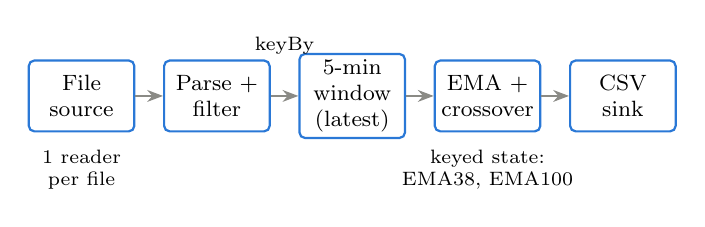
\begin{tikzpicture}[
  node distance=3.5mm,
  op/.style={draw=s1, thick, rounded corners=2pt, align=center,
             font=\footnotesize, minimum height=9mm, inner sep=2pt, text width=12mm},
  arr/.style={-{Stealth[length=2mm]}, muted, thick},
]
\node[op] (src) {File\\source};
\node[op, right=of src] (prs) {Parse +\\filter};
\node[op, right=of prs] (win) {5-min\\window\\(latest)};
\node[op, right=of win] (ema) {EMA +\\crossover};
\node[op, right=of ema] (snk) {CSV\\sink};
\draw[arr] (src) -- (prs);
\draw[arr] (prs) -- node[above, font=\scriptsize, text=black, yshift=4mm]{keyBy} (win);
\draw[arr] (win) -- (ema);
\draw[arr] (ema) -- (snk);
\node[below=1mm of ema, font=\scriptsize, align=center] {keyed state:\\EMA38, EMA100};
\node[below=1mm of src, font=\scriptsize, align=center] {1 reader\\per file};
\end{tikzpicture}
\caption{Dataflow of the job. The parse step is chained to the source.
Everything after \texttt{keyBy(symbol)} runs per key.}\label{fig:pipeline}
\end{figure}

\paragraph{Source and parsing.} Flink's \texttt{FileSource} reads the CSV
files line by line. A chained flat-map parses each line and
normalises it to (symbol, exchange from the symbol suffix, price, event time in
epoch milliseconds), dropping non-price rows. Since only
20\,\% of lines are price events, filtering before the shuffle removes most
of the network traffic.

\paragraph{Windowing (Q1).} Events are keyed by symbol and assigned to
5-minute tumbling event-time windows. We use an incremental \texttt{reduce}
that keeps only the event with the latest timestamp, so each open window holds
one event per symbol. A \texttt{ProcessWindowFunction} runs once per
(symbol, window) when the window fires.

\paragraph{EMA state and crossover (Q2).} The window function keeps EMA38 and
EMA100 in keyed \texttt{ValueState}, so the averages carry over from one window
to the next and are partitioned together with the key. Windows of one key fire
in event-time order, so the state is updated in the correct order. A buy
advisory is emitted when $\mathit{EMA}_{38} > \mathit{EMA}_{100}$ now and
$\mathit{EMA}_{38,\mathit{prev}} \le \mathit{EMA}_{100,\mathit{prev}}$; sell is
symmetric. This is the literal rule of the specification, confirmed by the
instructor, and our primary result: 24,836 advisories for the full week. It
also fires when the previous EMAs were \emph{equal}, which happens in a
symbol's second window, right after seeding. As an extra analysis of these
4,847 equal-start signals (19.5\,\%), a \texttt{--strict-crossover} option
requires a strict previous inequality; it yields 19,989.

\paragraph{Watermarks and determinism.} Within a file, event times are nearly
in order: no price row is more than 64.8\,s behind the latest event time seen
before it in its file. 99.9\,\% are at most 0.40\,s behind; only 5,442 of
59.4M rows (0.009\,\%) lag by more than 1\,s, 11 by more than 1 minute and
none by more than 6 minutes (\texttt{DisorderReport}). The exception is the
5,506 placeholder rows, about 18\,h behind (Section~\ref{sec:cleaning}).
Watermarks are generated per reader, and at 8 workers each file has its own
reader, so a tolerance of about 65\,s would have made no row late except the
placeholder rows (derived from these lags, not run). Across files, event times
interleave, since the files are read concurrently. We use
a bounded-out-of-orderness watermark with a tolerance of 200\,h, which is
longer than the dataset, so no event is ever late and all windows fire at the
end of input. Together with the deterministic latest-event rule, this makes the
output independent of parallelism and of read order, which we verify for every
configuration (Section~\ref{sec:correct}). A smaller tolerance makes the job
emit results sooner; a \texttt{--late-output} option then writes late events to
a side output instead of dropping them silently.

\section{Implementation and Optimisations}
The job is about 520 lines of Java (\texttt{Job.java}, \texttt{Parser.java})
and runs as a fat jar in Flink's local mini-cluster. Two changes gave most of
the single-worker speed:
\begin{itemize}
\item \emph{Parser.} The first parser split every line into all 39 fields and
  parsed timestamps through \texttt{java.time}. The new parser scans for the
  four needed columns only and parses timestamps by hand. It matched the old
  parser on 3M fuzzed lines and on the full outputs.
\item \emph{Garbage collector.} The job allocates many short-lived strings, and
  the throughput-oriented Parallel GC was about 25\,\% faster than the default G1.
\end{itemize}
Section~\ref{sec:ablation} quantifies both effects on the final code.

\section{Evaluation}\label{sec:eval}

\paragraph{Setup.} All runs use one laptop with an Intel Core i5-12450H
(4 performance cores with 2 threads each, plus 4 efficiency cores: 12 hardware
threads; WSL2 presents them as six identical two-thread cores), Windows 11 with
WSL2 (Ubuntu, 7.6\,GB memory available to Linux), the
data on the local SSD, OpenJDK 11.0.32, Flink 1.20.1, and
\texttt{-Xmx5g -XX:+UseParallelGC}.
Runtime is the wall-clock time of the whole process, including JVM and Flink
start-up (a few seconds), measured with \texttt{/usr/bin/time}. Each value is
the median of three runs; runs of different configurations are interleaved to
spread background noise. Run-to-run variation is up to $\pm$15\,\% (ranges in
Table~\ref{tab:speedup}).

\subsection{Correctness}\label{sec:correct}
The job computes 1,857,457 window results and 24,836 crossovers for the full
week. Results are compared key by key with \texttt{compare\_runs.py}: outputs at
parallelism 1, 2, 4 and 8, with both source implementations, with both parsers,
and with the input split into 8 chunks per day are all identical. On a
20-minute slice we checked the EMA values against an independent PyFlink
implementation of the same formulas. A JUnit test (10 cases) runs the job
in-process at parallelism 1 and 2 with both crossover rules on a synthetic
file with real BUY and SELL crossings, an equal-start signal, a constant price,
rows without a price or trading date, an out-of-order event and timestamp ties
with different prices, and compares every window with an independent
plain-loop implementation of the specification. Three injected bugs (a wrong
comparison, keeping the first event, letting the earlier line win a tie) all
make it fail.

\paragraph{Rounding.} The update $P\alpha + \mathit{EMA}_\mathit{prev}(1-\alpha)$
is not exact in floating point: for a constant price of 50, EMA38 becomes
49.999999999999986 while EMA100 stays 50, so the literal rule can fire on a
difference of $10^{-15}$. In the full week, 594 literal signals (2.4\,\%) are of
this kind (all equal-start signals, which the strict rule removes), and 260
strict signals (1.3\,\%) start from EMAs that differ only by rounding. The form
$\mathit{EMA}_\mathit{prev} + \alpha(P-\mathit{EMA}_\mathit{prev})$ would be
exact for constant prices; we did not re-run the job with it.

\paragraph{EMA starting value.}\label{sec:emainit} With the specification's
zero start (\texttt{--ema-init zero}), every symbol gets a BUY in its first
window, none has an advisory in windows 1--99 while the EMAs ramp up, and EMA38
needs a median of 88 windows (about 7\,h) to come within 1\,\% of the price;
1,523 symbols never do. It gives 11,355 advisories against our 24,836
(\texttt{docs/EXPERIMENTS.md}, Section~2).

\subsection{Scalability with parallelism}
Table~\ref{tab:speedup} and Figure~\ref{fig:speedup} show runtime and speedup
for 4 and 7 days. The speedup is sub-linear and levels off: 1.90$\times$ at 8
workers for 7 days. On 4 days, 8 workers are no faster than 4. At 8 workers the
job processes 5.0M CSV lines/s, or 1.04M price events/s.

\begin{table}[t]
\caption{Runtime (median of 3, min--max in brackets) and speedup.}\label{tab:speedup}
\begin{tabular}{rrrrr}
\toprule
 & \multicolumn{2}{c}{4 days (19\,GB)} & \multicolumn{2}{c}{7 days (24\,GB)} \\
Workers & Time (s) & Speedup & Time (s) & Speedup \\
\midrule
1 & 81.3 {\scriptsize(79--83)} & 1.00 & 108.8 {\scriptsize(98--111)} & 1.00 \\
2 & 62.2 {\scriptsize(55--63)} & 1.31 &  77.4 {\scriptsize(70--88)} & 1.40 \\
4 & 47.7 {\scriptsize(44--50)} & 1.71 &  66.0 {\scriptsize(62--86)} & 1.65 \\
8 & 49.6 {\scriptsize(49--58)} & 1.64 &  57.3 {\scriptsize(55--73)} & 1.90 \\
\bottomrule
\end{tabular}
\end{table}

\begin{figure}[t]
\centering
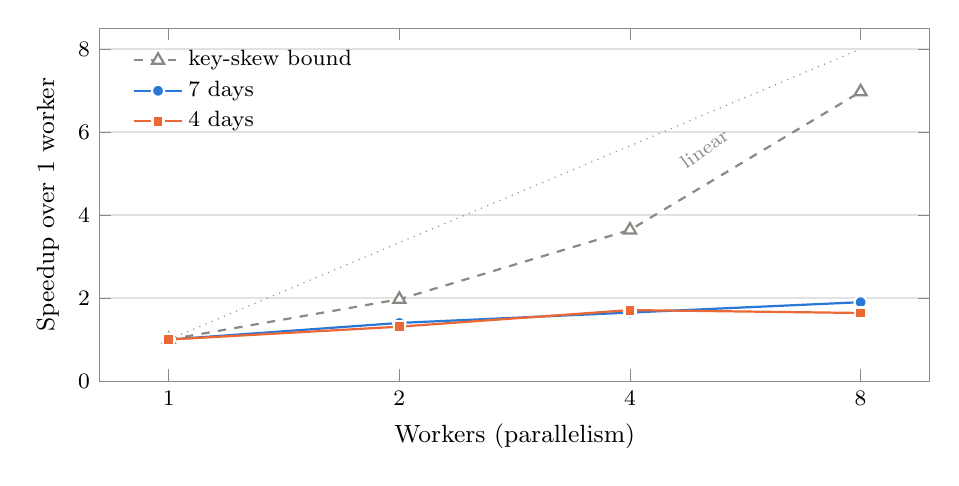
\begin{tikzpicture}
\begin{axis}[
  height=0.5\columnwidth,
  xmode=log, log basis x=2, xtick={1,2,4,8}, xticklabels={1,2,4,8},
  xlabel={Workers (parallelism)}, ylabel={Speedup over 1 worker},
  ymin=0, ymax=8.5, ytick={0,2,4,6,8},
  legend pos=north west,
]
\addplot[muted, thin, dotted, domain=1:8, samples=2, forget plot] {x};
\node[font=\scriptsize, text=muted, rotate=36] at (axis cs:5.0,5.6) {linear};
\addplot[muted, thick, dashed, mark=triangle*, mark size=2.5pt,
         mark options={solid, fill=white}]
  coordinates {(1,1) (2,1.97) (4,3.64) (8,6.97)};
\addlegendentry{key-skew bound}
\addplot[s1, thick, mark=*, mark size=2.2pt, mark options={draw=white}]
  coordinates {(1,1) (2,1.40) (4,1.65) (8,1.90)};
\addlegendentry{7 days}
\addplot[s2, thick, mark=square*, mark size=2.0pt, mark options={draw=white}]
  coordinates {(1,1) (2,1.31) (4,1.71) (8,1.64)};
\addlegendentry{4 days}
\end{axis}
\end{tikzpicture}
\caption{Measured speedup against the best speedup that key skew alone would
allow. The gap shows that skew is not the limit.}\label{fig:speedup}
\end{figure}

\subsection{Why the speedup levels off}
\paragraph{Key skew and the long tail --- not the limit.} With Flink's own
key-group assignment, the busiest worker receives 50.8, 27.5 and 14.3\,\% of
the price events at 2, 4 and 8 workers, which would still allow 1.97, 3.64 and
6.97$\times$ (Figure~\ref{fig:speedup}). The load has a long tail rather than a
few heavy keys: the busiest symbol holds 0.27\,\% of the events, the top 100
hold 26.9\,\%, and 306 symbols (6\,\%) cover half.

\paragraph{Window and EMA work --- small.} Runs restricted to one exchange
still read and parse every file: NL (10\,\% of the events) takes 72\,s against
86\,s for all exchanges with one worker, so the window and EMA stage costs
roughly 14\,s (8\,s with eight workers). Every exchange scales by
1.7--2.0$\times$ at 8 workers.

\paragraph{One reader per file --- the likely limit.} \texttt{FileSource} with a
text-line format reads each file with one worker, and the week has five large
files, so the run cannot finish before the largest file (5.5\,GB) has been read
by one thread. With 8 workers that day alone takes 31\,s on 2.2 cores, and
seven days take only 1.7$\times$ longer for 4.5$\times$ more data. The process
uses 7.6--7.8 of 12 hardware threads, only 8 of which are performance cores.
Pinned to 1--12 CPUs, the runtime falls from 161\,s to 43.7\,s (3.7$\times$)
while the CPU time rises 2.2$\times$. Splitting each day into 8 files used
almost 10 cores but did not shorten the run (Table~\ref{tab:ablation}), so
beyond the reader the shared hardware (4 performance cores, memory bandwidth,
WSL2's file layer) appears to be the limit; we did not measure this directly.
The per-exchange, volume and CPU-limit tables are in
\texttt{docs/EXPERIMENTS.md} in the repository (Section~3).

\subsection{Ablation}\label{sec:ablation}
Table~\ref{tab:ablation} changes one factor at a time from the final
configuration (full week, 8 workers). It was run in a separate session, so its
baseline differs from Table~\ref{tab:speedup} by about 10\,\%. Every
configuration produced identical output.

\begin{table}[t]
\caption{Ablation, 7 days, 8 workers (median of 3 runs).}\label{tab:ablation}
\begin{tabular}{lrrrr}
\toprule
Change from baseline & Time & Rel. & CPU & Memory \\
\midrule
None (baseline)$^\ast$       &  50.8\,s & 1.00 & 785\,\% & 2.7\,GB \\
Original split-based parser  & 108.5\,s & 2.13 & 679\,\% & 2.8\,GB \\
G1 GC (JVM default)          &  59.1\,s & 1.16 & 822\,\% & 4.7\,GB \\
Legacy splittable source     &  81.1\,s & 1.60 & 588\,\% & 2.7\,GB \\
Each day split into 8 files  &  49.8\,s & 0.98 & 986\,\% & 2.8\,GB \\
Object reuse enabled         &  49.9\,s & 0.98 & 819\,\% & 2.7\,GB \\
\bottomrule
\multicolumn{5}{l}{\footnotesize Baseline: fast parser, Parallel GC, FileSource, one file per day.}\\
\multicolumn{5}{l}{\footnotesize $^\ast$One baseline run stalled (584\,s at 73\,\% CPU) and was repeated.}\\
\end{tabular}
\end{table}

The parser matters most: the original parser makes the whole job 2.1$\times$
slower, which confirms that parsing dominates. Parallel GC is 16\,\% faster
than G1 and uses 1.7$\times$ less memory. Object reuse and splitting the files
have no measurable effect (2\,\% is within noise); the deprecated splittable
legacy source is 1.6$\times$ slower.

\section{Visualisation}\label{sec:viz}
To inspect the results we built a static web page (vanilla JavaScript, no
server) from the job's output (Figure~\ref{fig:viz}). It shows EMA38, EMA100
and the signals per symbol, with zoom, a literal/strict toggle, a day $\times$
hour heat map of crossings, and the benchmark results. It revealed two problems
that the aggregate counts hid: the 01:00 index window
(Section~\ref{sec:data}) and \emph{flat} symbols. 1,004 symbols move less than
0.5\,\% in EMA38 over the week, and two of them were the top crossers, whose
crossings came from single-tick price changes. The page draws only non-flat
symbols by default; all totals still include every symbol.

\begin{figure}[t]
\centering
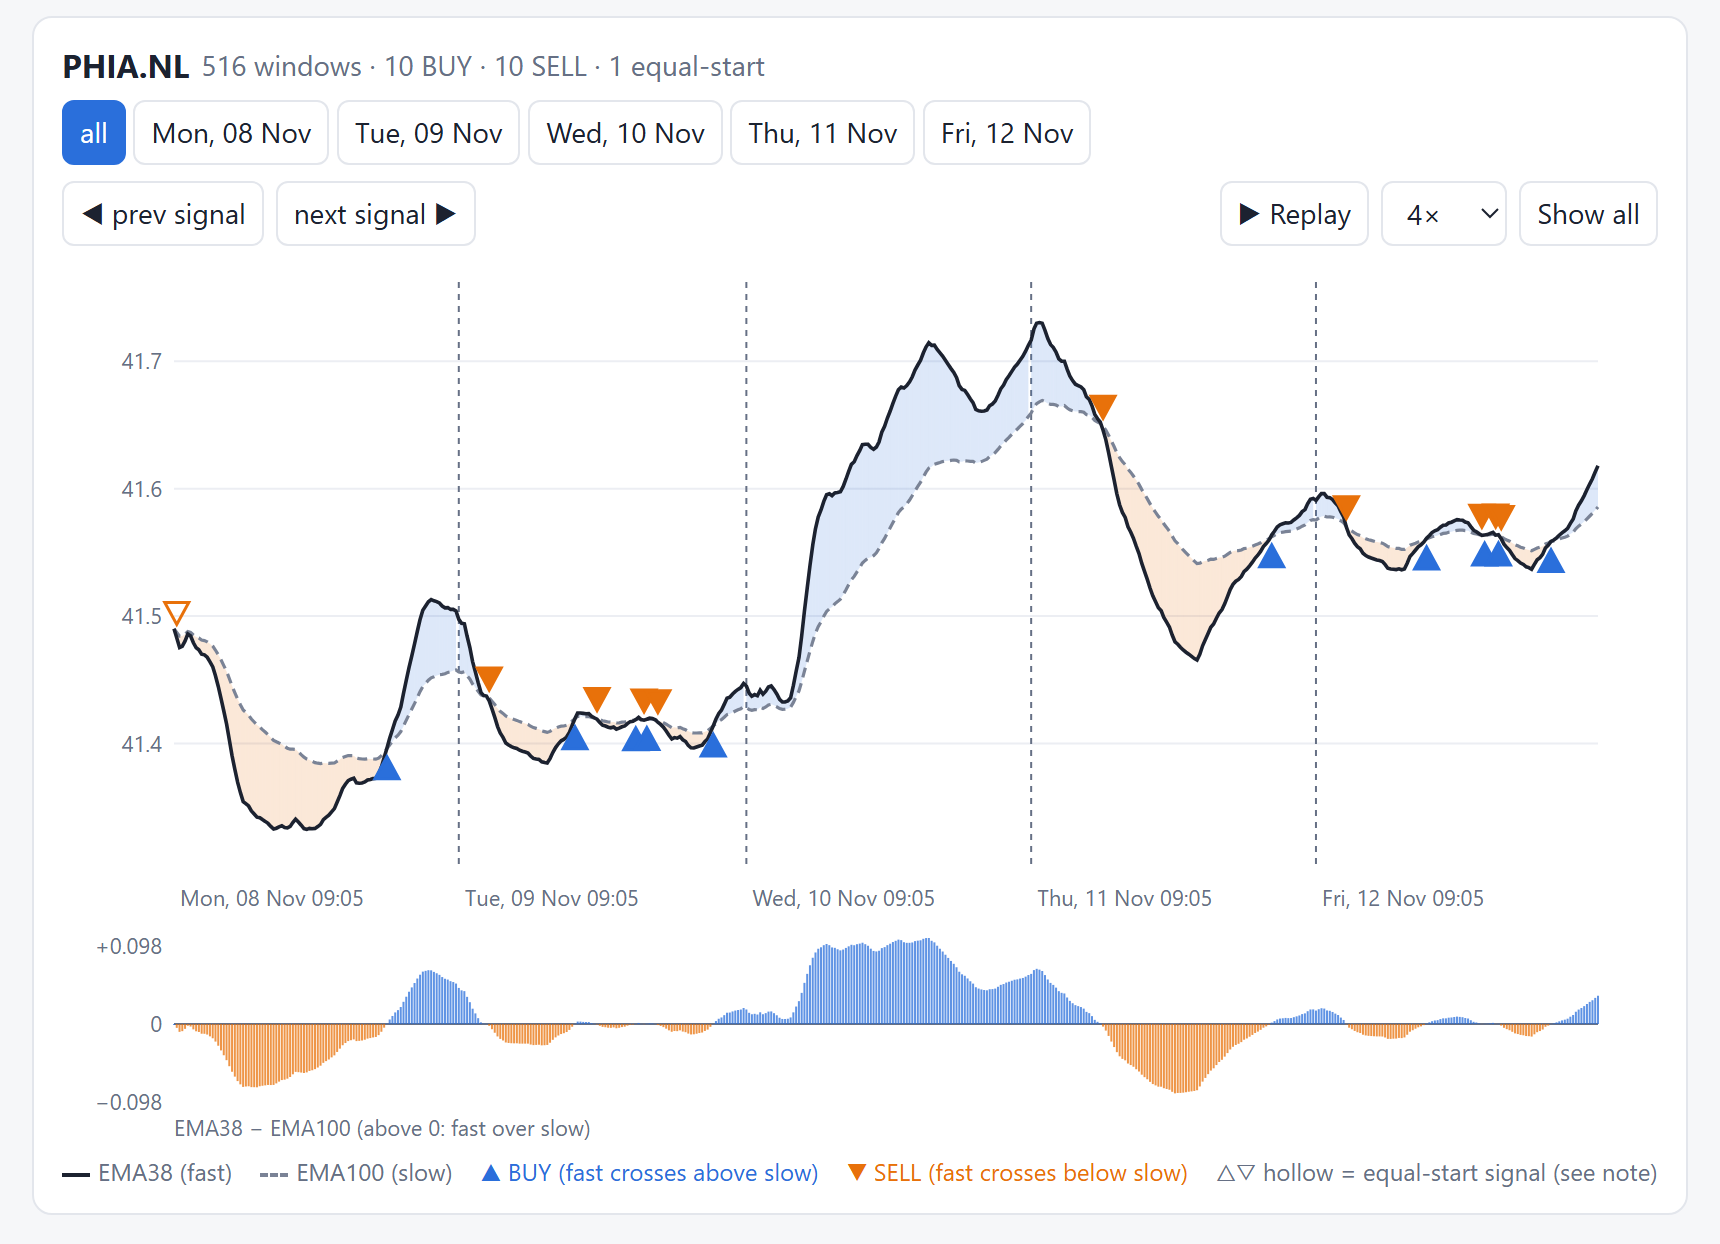
\includegraphics[width=\columnwidth]{figures/viz-chart.png}
\caption{The result explorer for Philips (PHIA.NL): EMA38 (solid) and EMA100
(dashed) per 5-minute window, BUY (blue) and SELL (orange) triangles, one hollow equal-start signal, and the
EMA spread below.}\label{fig:viz}
\end{figure}

\section{Discussion and Limitations}\label{sec:discussion}
\paragraph{Late events and tolerance.} On the full week, tolerances of 200\,h
and 24\,h give no late events; 6\,h, 1\,h and 0.1\,h all give exactly the
5,506 placeholder rows as late, with the same result as dropping them
(Section~\ref{sec:cleaning}). Our main run uses 200\,h because it makes the
results independent of parallelism and reading order; a streaming deployment
could use a tolerance of minutes.

\begin{table}[t]
\caption{Paced replay of 11 November (tolerance 0.1\,h, 368,727 results;
latency in ms). Excess: measured latency minus the built-in wait (event time
from the window's last event to window end $+$ tolerance, divided by $S$).
$^\ast$Later runs, with the machine about 2.4$\times$ slower.}\label{tab:paced}
\small
\setlength{\tabcolsep}{4pt}
\begin{tabular}{lrrrrr}
\toprule
 & & \multicolumn{2}{c}{Measured} & \multicolumn{2}{c}{Excess} \\
$S$ & Time (s) & median & p99 & median & p99 \\
\midrule
60              & 938.7 & 6,397 & 11,051 & 145 & 286 \\
300             & 190.7 & 1,381 &  2,347 & 120 & 239 \\
1500            &  41.2 &   406 &    576 & 147 & 272 \\
unpaced         &  22.7 &   313 &    614 & 313 & 614 \\
3000$^\ast$     &  56.9 &   625 &  1,085 & 498 & 904 \\
6000$^\ast$     &  58.6 &   652 &  1,384 & 588 & 1,320 \\
unpaced$^\ast$  &  53.8 &   593 &  1,459 & 593 & 1,459 \\
\bottomrule
\end{tabular}
\end{table}

\paragraph{Latency.} With \texttt{--latency-log}, every result records the
time from the arrival of its window's last event to its emission. Read at full
speed, the input is a backlog, and the full week gives a median of 40\,s that
reflects the length of the run, not latency. A paced replay
(\texttt{--replay-speed}~$S$) therefore releases each event when
$\textit{start} + V/S$ has passed, $V$ being the event time elapsed so far
(jumps over 10 minutes count as 10); the arrival is stamped at release.
Table~\ref{tab:paced} replays 11 November (11.8M events, no placeholder rows,
one day file read by one reader). A window fires only when event time passes
its end plus the tolerance, so its last event waits 6--11 minutes of event
time, 6--11\,s at $S{=}60$: the tolerance and window size set the latency. The
excess over this wait stays at a median of 120--150\,ms up to $S{=}1500$ (287k
events/s), consistent with the 200\,ms watermark interval. At $S{=}3000$ and
$6000$ the runs took as long as an unpaced run and the excess grew: the
pipeline saturates. These runs were made with the machine about 2.4$\times$
slower, so where saturation starts in the faster state is an extrapolation
(near $S \approx 3{,}000$). With the probe off, the probe code costs about
5\,\% (52.7 vs 50.0\,s; the throughput numbers above predate it). Full tables
are in \texttt{docs/EXPERIMENTS.md} in the repository (Section~4).

\paragraph{Interpretation choices.} The crossover rule and the window price
are fixed by the instructor. The strict rule (4,847 fewer signals, 19.5\,\%) is
an extra analysis, and rounding moves another 1--2\,\% of the signals
(Section~\ref{sec:correct}). The handling of rows without a trading date and of
late events is our own choice; both change which windows exist.

\paragraph{Single machine.} All measurements are from one laptop running
Flink's mini-cluster, so the shuffle never crosses a network. On a cluster with
one disk per node, the per-file reader would scale with the number of nodes,
while the shuffle of 59.4M small records would add network cost.

\section{Conclusion}
A small Flink job computes both DEBS 2022 queries on a full week of tick data
in under a minute on a laptop, with results identical at every parallelism
level. Profiling showed that windowing and EMA state are cheap and key skew is
mild. The cost lies in reading and parsing 24\,GB of text, and Flink's
file-level source parallelism limits how far that step can be spread. In a
paced replay, the pipeline adds about 0.15\,s to the latency that the window
size and tolerance impose.

\begin{acks}
% TODO: individual contributions, if required by the course.
\end{acks}

\bibliographystyle{ACM-Reference-Format}
\bibliography{references}

\end{document}
